\documentclass[tikz,border=4mm]{standalone}

\usepackage{amsmath,amssymb}
\usetikzlibrary{calc}

\newcommand{\Xc}{\mathcal{X}}

\begin{document}

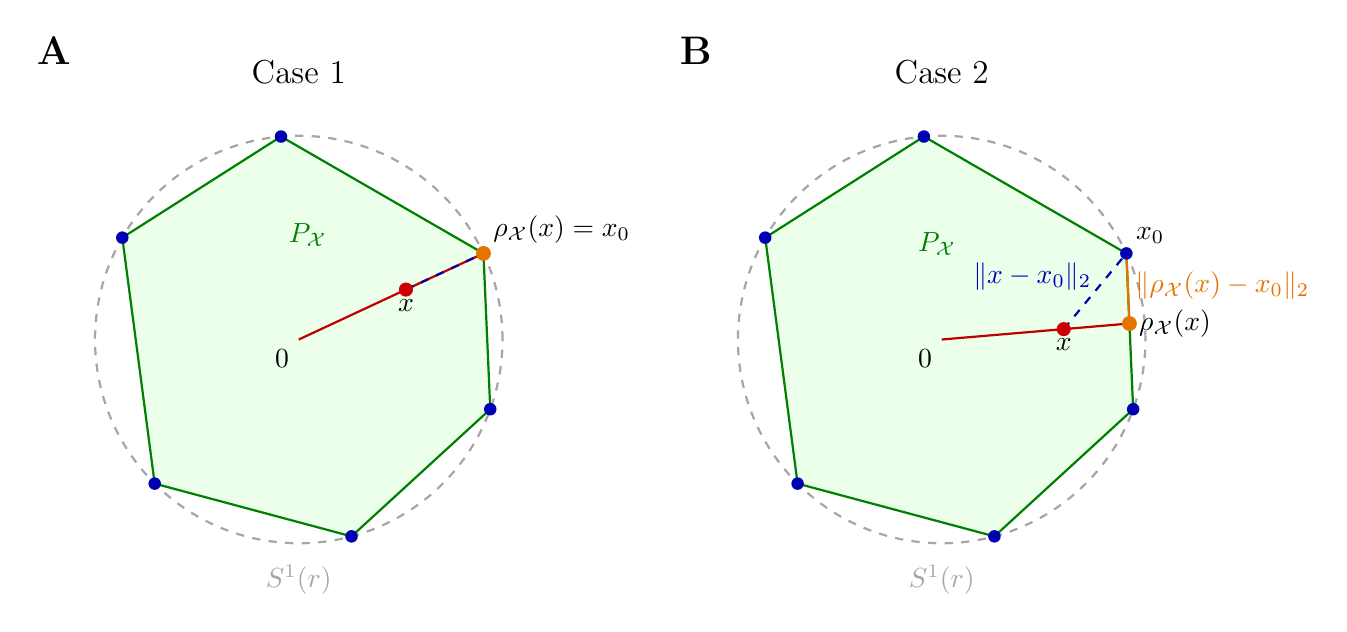
\begin{tikzpicture}[scale=1.15]

\tikzset{
  circleguide/.style={
    gray!70,
    dashed,
    thick
  },
  polygonfill/.style={
    fill=green!8,
    draw=green!50!black,
    thick
  },
  xsetpoint/.style={
    circle,
    fill=blue!70!black,
    inner sep=1.6pt
  },
  xpoint/.style={
    circle,
    fill=red!80!black,
    inner sep=1.8pt
  },
  rhopoint/.style={
    circle,
    fill=orange!90!black,
    inner sep=1.9pt
  },
  radial/.style={
    red!75!black,
    thick
  },
  aux/.style={
    blue!70!black,
    dashed,
    thick
  },
  shortseg/.style={
    orange!90!black,
    thick
  }
}

% Common position of panel labels
\def\panelLabelX{-3.0}
\def\panelLabelY{3.45}

%%%%%%%%%%%%%%%%%%%%%%%%%%%%%%%%%%%%%%%%%%%%%%%%%%%%%%%%%%%%
%% Panel A: rho_X(x) = x_0
%%%%%%%%%%%%%%%%%%%%%%%%%%%%%%%%%%%%%%%%%%%%%%%%%%%%%%%%%%%%
\begin{scope}[xshift=0cm]

% Panel label
\node[
  anchor=north west,
  font=\bfseries\Large
] at (\panelLabelX,\panelLabelY) {A};

% Origin and radius
\coordinate (O1) at (0,0);
\def\R{2.25}

% Points on the circle
\coordinate (A1) at ({\R*cos(150)},{\R*sin(150)});
\coordinate (B1) at ({\R*cos(95)},{\R*sin(95)});
\coordinate (C1) at ({\R*cos(25)},{\R*sin(25)});
\coordinate (D1) at ({\R*cos(-20)},{\R*sin(-20)});
\coordinate (E1) at ({\R*cos(-75)},{\R*sin(-75)});
\coordinate (F1) at ({\R*cos(-135)},{\R*sin(-135)});

% Polygon P_X
\draw[polygonfill]
  (A1)--(B1)--(C1)--(D1)--(E1)--(F1)--cycle;

% Ambient circle S^1(r)
\draw[circleguide] (O1) circle (\R);

% Choose x_0 = rho_X(x)
\coordinate (X01) at (C1);
\coordinate (X1) at ($(O1)!0.58!(X01)$);

% Radial and auxiliary lines
\draw[radial] (O1)--(X01);
\draw[aux] (X1)--(X01);

% Plot all points in X
\foreach \P in {A1,B1,C1,D1,E1,F1}{
  \node[xsetpoint] at (\P) {};
}

% Plot x and rho_X(x)
\node[xpoint] at (X1) {};
\node[rhopoint] at (X01) {};

% Labels
\node[below left] at (O1) {$0$};
\node[below] at (X1) {$x$};
\node[above right] at (X01)
  {$\rho_{\Xc}(x)=x_0$};

\node at (0,2.95)
  {\large Case 1};

\node[green!50!black] at (0.1,1.15)
  {$P_{\Xc}$};

\node[gray!70] at (0,-2.65)
  {$S^1(r)$};

\end{scope}

%%%%%%%%%%%%%%%%%%%%%%%%%%%%%%%%%%%%%%%%%%%%%%%%%%%%%%%%%%%%
%% Panel B: rho_X(x) != x_0
%%%%%%%%%%%%%%%%%%%%%%%%%%%%%%%%%%%%%%%%%%%%%%%%%%%%%%%%%%%%
\begin{scope}[xshift=7.1cm]

% Panel label
\node[
  anchor=north west,
  font=\bfseries\Large
] at (\panelLabelX,\panelLabelY) {B};

% Origin and radius
\coordinate (O2) at (0,0);
\def\R{2.25}

% Same points on the circle as in Case 1
\coordinate (A2) at ({\R*cos(150)},{\R*sin(150)});
\coordinate (B2) at ({\R*cos(95)},{\R*sin(95)});
\coordinate (C2) at ({\R*cos(25)},{\R*sin(25)});
\coordinate (D2) at ({\R*cos(-20)},{\R*sin(-20)});
\coordinate (E2) at ({\R*cos(-75)},{\R*sin(-75)});
\coordinate (F2) at ({\R*cos(-135)},{\R*sin(-135)});

% Polygon P_X
\draw[polygonfill]
  (A2)--(B2)--(C2)--(D2)--(E2)--(F2)--cycle;

% Ambient circle S^1(r)
\draw[circleguide] (O2) circle (\R);

% Choose rho_X(x) on the edge [C2,D2]
\coordinate (RHO2) at ($(C2)!0.45!(D2)$);

% Choose x on the ray from the origin through rho_X(x)
\coordinate (X2) at ($(O2)!0.65!(RHO2)$);

% Choose the nearest point x_0 in X
\coordinate (X02) at (C2);

% Radial and comparison segments
\draw[radial] (O2)--(RHO2);
\draw[aux] (X2)--(X02);
\draw[shortseg] (RHO2)--(X02);

% Plot all points in X
\foreach \P in {A2,B2,C2,D2,E2,F2}{
  \node[xsetpoint] at (\P) {};
}

% Plot x and rho_X(x)
\node[xpoint] at (X2) {};
\node[rhopoint] at (RHO2) {};

% Labels
\node[below left] at (O2) {$0$};
\node[below] at (X2) {$x$};
\node[right] at (RHO2)
  {$\rho_{\Xc}(x)$};
\node[above right] at (X02)
  {$x_0$};

\node at (0,2.95)
  {\large Case 2};

\node[green!50!black] at (-0.05,1.05)
  {$P_{\Xc}$};

\node[gray!70] at (0,-2.65)
  {$S^1(r)$};

% Distance labels
\node[
  blue!70!black,
  font=\normalsize
] at (1,0.7)
  {$\|x-x_0\|_2$};

\node[
  orange!90!black,
  font=\normalsize
] at (3.1,0.6)
  {$\|\rho_{\Xc}(x)-x_0\|_2$};

\end{scope}

\end{tikzpicture}

\end{document}